\chapter{流形}
我们从几何学的源头开始, 找寻一些经典几何学的关键要素, 然后在这些要素之上来搭建我们的舞台: 微分流形.
\section{几何学是什么?}
现代几何学源于古希腊.
在古希腊语中, ``几何学''一词为γεωμετρία \textit{(geōmetría)}, 意为测量大地.
这反映了早期几何学主要是对长度, 面积, 体积, 角度的经验性原理的收集, 主要用于满足实用性用途.
直至今日, 初步的几何学教学仍然是从对几何体的大小的直观认识开始的.
因此几何学的一个经典要件就是\emph{度量}.

Euclid所著的\textit{Elements} (汉语中通常称作《几何原本》) 是古希腊几何的代表.
他在\textit{Elements}的开篇引入了这样的一条公理:
\begin{quotation}
    {\bfseries 公理}4.\ 彼此能重合的物体是全等的.
\end{quotation}
然后第一个引用了这条公理的命题是
\begin{quotation}
    {\bfseries 命题}4.\ 如果两个三角形中, 一个的两边分别等于另一个的两边, 而且这些线段所夹的角相等.
    那么它们的底边等于底边, 这样其余的角也等于相应的角, 即那些等边所对应的角.
    \begin{flushright}
        (译文引自~\parencite{Euclid_Elem})
    \end{flushright}
\end{quotation}
在这最原始的直觉中, ``重合''蕴含了运动的概念, 而边角的相等则蕴含了不变量的概念.
因此, 几何学的另一个经典要件就是\emph{变换与不变量}.

古希腊的几何学主要研究直线与圆锥曲线.
到了微积分发明之后, 数学家可以使用微积分的工具来研究更一般的几何体了.
Leibniz通过密切圆引入了曲线的曲率, Bernoulli与Euler研究了曲面的法曲率与测地线.
对``曲''的研究正式进入了几何学之中.
1827年, Gauss在论文\textit{Disquisitiones generales circa superficies curvas} (关于曲面的一般研究) 中证明了``Gauss绝妙定理'' (Theorema Egregium).
从此一种观念开始进入几何学: 我们可以研究抽象的几何体, 而不考虑它在欧氏空间中的实现.
进而不久非欧几何便产生了.

回到几何学的两个要件上.
有了以上基础, 1854年Riemann写作了论文\textit{\"{U}ber die hypothesen welche der Geometrie zu Grunde liegen} (论奠定几何学基础的假设), 正式引入了Riemann度量与流形的概念 (之后的笔记中我们会详细解释这两个概念).
同时, 19世纪正在经历一个射影几何的复兴潮, 当时正在流行使用射影变换的方法研究射影几何.
于是在1893年F.\ Klein发表了对整个几何学的``总结性''综述\textit{Vergleichende Betrachtungen \"{u}ber neuere geometrische Forschungen} (关于近代几何学研究的比较考察).
文章中提到几何学的目的在于
\begin{quotation}
    给定一个流形和其上的变换群, 发展关于这个群的不变量理论.
    \begin{flushright}
        (\parencite{Klein_Erlangen}, 自译)
    \end{flushright}
\end{quotation}

自此, 经典几何学的舞台已经搭好.
但我们还有一个问题: \label{intro_sect}
\begin{pro}
    微分几何是什么?
\end{pro}
接下来我们开始慢慢搭微分几何的舞台.

\section{微分流形}
由于我们要在一般的几何体上处理问题, 所以我们要先引入\textit{流形}的概念.
在数学分析的课程中, 我们学习过了$\mathbb{R}^n$的$k$维子流形的概念 (例如在~\parencite{Zorich_MathAnal}~的第8章).
$k$维子流形的概念是一个局部长得像$\mathbb{R}^k$的空间.
这启发我们给出一般流形的定义:
\begin{defn}
    一个$n$维\textbf{拓扑流形}$M$是一个第二可数, Haussdorf的拓扑空间, 并且$M$的每一点都有一个邻域同胚于$\mathbb{R}^n$中的一个开集.
\end{defn}
\begin{rem}
    拓扑流形定义中的第二可数与Haussdorf这两个条件目前看不出来有什么作用, 但这两个条件能够保证\textit{单位分解定理}这个重要的工具成立, 之后遇到了我们会再讨论这一点.
    此外, 给出上述定义之后我们需要证明$n$维拓扑流形是良定义的, 即证明$\mathbb{R}^n$与$\mathbb{R}^m$在$m\neq n$时不同胚, 但这需要用到代数拓扑的工具 (参考~\parencite[定理 17.26]{Lee_IntroSmMani}, 那里用的是de Rham理论).
    不过证明微分流形是良定义的会相对比较简单, 之后我们会处理这件事情.
\end{rem}
由于我们不太需要关心流形的拓扑, 所以以上定义对微分几何来说其实并不是特别重要\footnote{也就是你不懂的话也不必深究的意思.}.
对流形而言, 重要的是它上面的\textit{微分结构}.
\begin{defn}
    设$M$是$n$维拓扑流形.
    设$\{U_\alpha\}_{\alpha\in A}$是$M$的一族开覆盖, 满足其中每个开集都同胚于$\mathbb{R}^n$中的开集.
    每个开集对应的同胚映射$\varphi_\alpha:U_\alpha\to\mathbb{R}^n$被称为\textbf{坐标卡}.
    如果两个坐标卡$\varphi_\alpha,\varphi_\beta$满足$\varphi_\alpha\circ\varphi_\beta^{-1},\varphi_\beta\circ\varphi_\alpha^{-1}$在其定义域上是$C^\infty$的, 那么称这两个坐标卡相容.
    如果这一族开覆盖的任意两个坐标卡相容, 那么这一族开覆盖$\{U_\alpha\}_{\alpha\in A}$便称为$M$的一个\textbf{图册}.
    如果$M$的一个图册中无法再加入新的相容的坐标卡, 那么称这个图册是\textbf{极大}的.
    极大的图册构成$M$的一个\textbf{微分结构}.
    拥有微分结构的拓扑流形被称为\textbf{微分流形}.
\end{defn}
有时我们会将$\varphi_\beta\circ\varphi_\alpha^{-1}$称为\textbf{转移函数}.
我们有一张图可以用来直观地理解转移函数:
\begin{figure}[ht]
    \centering
    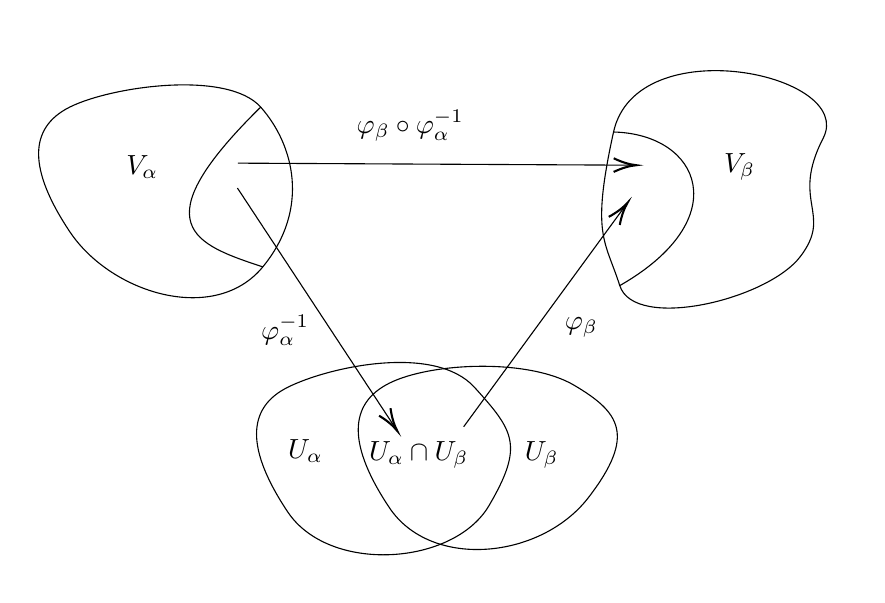
\begin{tikzpicture}[x=0.75pt,y=0.75pt,yscale=-1,xscale=1]
    %uncomment if require: \path (0,301); %set diagram left start at 0, and has height of 301

    %Shape: Polygon Curved [id:ds7545552056106698] 
    \draw   (50,45) .. controls (70,35) and (126,27) .. (142,45) .. controls (158,63) and (166,94) .. (143,122) .. controls (120,150) and (70,135) .. (50,105) .. controls (30,75) and (30,55) .. (50,45) -- cycle ;
    %Shape: Polygon Curved [id:ds5522702672450327] 
    \draw   (312,57) .. controls (323,7) and (429,29) .. (413,60) .. controls (397,91) and (418,96) .. (402,117) .. controls (386,138) and (322,153) .. (315,131) .. controls (308,109) and (301,107) .. (312,57) -- cycle ;
    %Curve Lines [id:da21169301483212177] 
    \draw    (142,45) .. controls (84,102) and (110,111) .. (143,122) ;
    %Curve Lines [id:da030881504774420643] 
    \draw    (312,57) .. controls (354,58) and (371,99) .. (315,131) ;
    %Shape: Polygon Curved [id:ds7639047336485658] 
    \draw   (155,180) .. controls (175,170) and (226,159) .. (245,180) .. controls (264,201) and (269,208) .. (252,237) .. controls (235,266) and (175,270) .. (155,240) .. controls (135,210) and (135,190) .. (155,180) -- cycle ;
    %Shape: Polygon Curved [id:ds6261763207033869] 
    \draw   (204,178) .. controls (224,168) and (271,166) .. (293,179) .. controls (315,192) and (323,203) .. (300,233) .. controls (277,263) and (224,268) .. (204,238) .. controls (184,208) and (184,188) .. (204,178) -- cycle ;
    %Straight Lines [id:da16391710195567155] 
    \draw    (239.8,199) -- (317.62,92.61) ;
    \draw [shift={(318.8,91)}, rotate = 126.18] [color={rgb, 255:red, 0; green, 0; blue, 0 }  ][line width=0.75]    (10.93,-3.29) .. controls (6.95,-1.4) and (3.31,-0.3) .. (0,0) .. controls (3.31,0.3) and (6.95,1.4) .. (10.93,3.29)   ;
    %Straight Lines [id:da31384654750788643] 
    \draw    (130.8,84) -- (206.7,199.33) ;
    \draw [shift={(207.8,201)}, rotate = 236.65] [color={rgb, 255:red, 0; green, 0; blue, 0 }  ][line width=0.75]    (10.93,-3.29) .. controls (6.95,-1.4) and (3.31,-0.3) .. (0,0) .. controls (3.31,0.3) and (6.95,1.4) .. (10.93,3.29)   ;
    %Straight Lines [id:da13626397217094843] 
    \draw    (131,72) -- (321,72.99) ;
    \draw [shift={(323,73)}, rotate = 180.3] [color={rgb, 255:red, 0; green, 0; blue, 0 }  ][line width=0.75]    (10.93,-3.29) .. controls (6.95,-1.4) and (3.31,-0.3) .. (0,0) .. controls (3.31,0.3) and (6.95,1.4) .. (10.93,3.29)   ;

    % Text Node
    \draw (76,67) node [anchor=north west][inner sep=0.75pt]   [align=left] {$\displaystyle V_{\alpha }$};
    % Text Node
    \draw (364,66) node [anchor=north west][inner sep=0.75pt]   [align=left] {$\displaystyle V_{\beta }$};
    % Text Node
    \draw (154,204) node [anchor=north west][inner sep=0.75pt]   [align=left] {$\displaystyle U_{\alpha }$};
    % Text Node
    \draw (268,205) node [anchor=north west][inner sep=0.75pt]   [align=left] {$\displaystyle U_{\beta }$};
    % Text Node
    \draw (193,205) node [anchor=north west][inner sep=0.75pt]   [align=left] {$\displaystyle U_{\alpha } \cap U_{\beta }$};
    % Text Node
    \draw (141,144) node [anchor=north west][inner sep=0.75pt]   [align=left] {$\displaystyle \varphi _{\alpha }^{-1}$};
    % Text Node
    \draw (287.3,145) node [anchor=north west][inner sep=0.75pt]   [align=left] {$\displaystyle \varphi _{\beta }$};
    % Text Node
    \draw (187,45) node [anchor=north west][inner sep=0.75pt]   [align=left] {$\displaystyle \varphi _{\beta } \circ \varphi _{\alpha }^{-1}$};
\end{tikzpicture}
    \caption{转移函数}
\end{figure}

\begin{eg}我们举几个微分流形的例子.
    \begin{enumerate}[(1)]
        \item $\mathbb{R}^n$, 以恒等映射$1_{\mathbb{R}^n}$为坐标卡.
        我们指出一点, 证明一个流形具有微分结构只需要找出一组图册就可以了, 这组图册对应的微分结构就是所有与图册相容的坐标卡的集合.
        一般将恒等映射所在的图册称为$\mathbb{R}^n$的\textbf{标准微分结构}.
        \item $\mathbb{R}$, 以$\varphi:u\mapsto u^3$为坐标卡.
        注意到$\varphi$是$\mathbb{R}$到自身的同胚, 从而决定了一个微分结构.
        但是$1_{\mathbb{R}}\circ\varphi^{-1}$在$u=0$处不可导, 因此这个微分结构与标准微分结构不相容.
        这说明了一个微分流形上的微分结构可以有不止一个.
        \item 单位球面$\mathbb{S}^n$, 南北两极的球极投影. 两个球极投影$p_N,p_S$分别满足
        \begin{gather*}
            p_N(x_1,x_2,\cdots,x_{n+1})=\frac{1}{1-x_{n+1}}(x_1,x_2,\cdots,x_n)\\
            p_S(x_1,x_2,\cdots,x_{n+1})=\frac{1}{1+x_{n+1}}(x_1,x_2,\cdots,x_n)
        \end{gather*}
        在截面上用简单的平面几何可以推出转移函数为$1_{\mathbb{R}^n}/|1_{\mathbb{R}^n}|^2$, 是光滑函数.
    \end{enumerate}
\end{eg}
由于我们主要关心曲线曲面论, 所以我们不在这里再举其他奇怪 (但是有趣) 的流形的例子了.
而作为流形的曲线与曲面, 我们将在后面子流形的部分讨论它们.

微分结构的一个很重要的作用是可以定义光滑函数.
\begin{defn}\label{smooth function 1}
    设$M$是微分流形, 函数$f:M\to\mathbb{R}$被称为是\textbf{光滑}的是指对任意$p\in M$, 都存在一个包含$p$的坐标卡$(U,\varphi)$使得$f\circ\varphi^{-1}$是$C^\infty$的.
\end{defn}

\begin{sym}
    我们用$C^\infty(M)$来表示$M$上全体光滑函数的集合, 在逐点定义的加法与乘法下, 这是一个$\mathbb{R}$-代数 (同时是交换环与$\mathbb{R}$-向量空间).
\end{sym}

在这一节的最后我们引入流形的定向的概念.
我们用$\d f$来表示一个可微映射$f$的微分, 即最佳近似线性映射.
\begin{defn}
    设$M$是微分流形, 如果它拥有一组图册满足任意转移函数的Jacobi行列式$\det\d(\varphi_\alpha\circ\varphi_\beta^{-1})>0$, 那么就称$M$为\textbf{可定向流形}, 这样的一组图册称为给出了$M$的一个\textbf{定向}; 否则称$M$为\textbf{不可定向流形}.
\end{defn}

\begin{eg}
    \begin{enumerate}[(1)]
        \item $\mathbb{R}^3$的一组基对应了一个坐标卡, 转移函数的行列式就是过渡矩阵的行列式.
        我们知道$\mathbb{R}^3$的基有左手系和右手系的区分, 右手系到右手系的过渡矩阵行列式为正, 右手系到左手系的过渡矩阵行列式为负.
        因此左手系和右手系分别决定了$\mathbb{R}^3$的一种定向, 这也是定向这一概念的来源.
        \item 如果流形$M$的一个图册中只有两个坐标卡, 那么$M$一定可定向:
        设这两个坐标卡是$(U_1,\varphi_1)$与$(U_2,\varphi_2)$, 如果$\det\d(\varphi_1\circ\varphi_2^{-1})>0$, 那么已经完成证明;
        否则我们复合一个$\mathbb{R}^n$上的反射变换$r$, 得到新的坐标卡$\varphi_3=r\circ\varphi_2:U_2\to\mathbb{R}^n$, 那么新的图册$\{(U_1,\varphi_1),(U_2,\varphi_3)\}$就满足$\det\d(\varphi_1\circ\varphi_3^{-1})=\det\d(\varphi_1\circ\varphi_2^{-1})\det{r^{-1}}>0$, 从而$M$可定向.
        \item 按照上面的判别法, 单位球面$\mathbb{S}^n$拥有两个球极投影构成的图册, 所以是可定向的.
    \end{enumerate}
\end{eg}

关于流形的定向有一个基础的结论:

\begin{prop}
    一个连通的可定向流形恰好有两个定向.
\end{prop}

\begin{proof}
    证明这个命题需要一些拓扑论证, 但我们不希望在这份笔记里出现太多的拓扑, 所以我们直接引用~\parencite[引理1.1.2]{Mei_Manifold}.
\end{proof}

事实上确实存在不可定向的流形, 比如大家熟悉的M\"{o}bius带, 我们在之后再来讨论这个例子.\label{sect_of_mani}

\section{切空间与微分映射}
用``切''的手段来研究流形是微分几何学的基本想法, 我们在这一节建立有关切的几个概念.
首先我们使用内蕴的方法定义切向量, 并定义切空间与切丛.
然后我们讨论切空间之间的微分映射, 以及通过链式法则得到的重要推论, 即维度的微分同胚不变性.

\subsection*{切向量与切空间}
在数学分析课程中, 我们会考虑由函数图像给定的曲面, 并使用这个函数的微分映射的像来定义切平面.
但是在一般的微分流形中, 我们没有办法先验地给坐标卡定义微分, 所以我们要寻找其他的办法来定义流形的切向量.

对于曲面$S$上$p$点处的一个切向量$v$, 我们可以找到一条曲线$c:I\to S$使得$p=c(0),v=c'(0)$ (这里的导数定义为逐分量求导).
为了去掉全空间, 我们考虑一个函数$f:S\to\mathbb{R}$, 那么由链式法则有
\[(f\circ c)'(0)=\langle\grad{f}(p),c'(0)\rangle\]
我们熟悉右侧是由切向量决定的方向导数.
由梯度与内积的线性性可知
\begin{equation}
    ((\lambda f+\mu g)\circ c)'(0)=\lambda(f\circ c)'(0)+\mu(g\circ c)'(0)\label{linearity}
\end{equation}
又由乘积函数的求导法则, 可以得到
\begin{equation}
    ((fg)\circ c)'(0)=(f\circ c)(0)(g\circ c)'(0)+(g\circ c)(0)(f\circ c)'(0)\label{leibniz}
\end{equation}
通过以上式子, 我们可以看出方向导数可以被$S$上的曲线决定, 从而并不需要全空间.

\begin{figure}[ht]
    \centering
    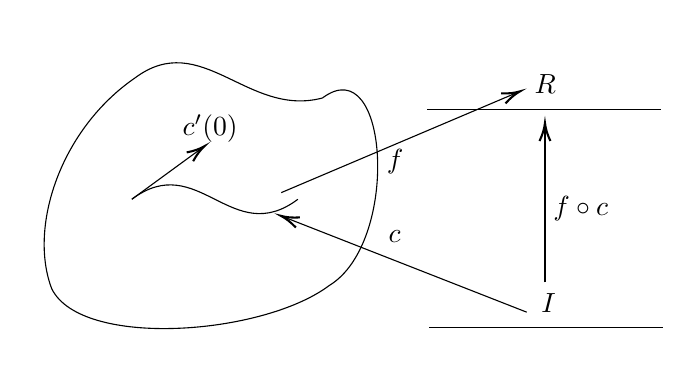
\begin{tikzpicture}[x=0.75pt,y=0.75pt,yscale=-0.8,xscale=0.8]
%uncomment if require: \path (0,300); %set diagram left start at 0, and has height of 300

%Curve Lines [id:da014063753011146707] 
\draw    (103.8,187) .. controls (89.6,150) and (108.8,91) .. (153.8,60) ;
%Curve Lines [id:da6854687890121294] 
\draw    (153.8,60) .. controls (193.8,30) and (221.8,84) .. (266.8,72) ;
%Curve Lines [id:da8800895461125313] 
\draw    (103.8,187) .. controls (121.8,223) and (230.8,215) .. (270.8,185) ;
%Curve Lines [id:da9135462557807166] 
\draw    (266.8,72) .. controls (306.8,42) and (313.8,159) .. (270.8,185) ;
%Curve Lines [id:da6496864524155734] 
\draw    (152,133) .. controls (192,103) and (212,163) .. (252,133) ;
%Straight Lines [id:da4417753278815133] 
\draw    (152,133) -- (194.19,102.18) ;
\draw [shift={(195.8,101)}, rotate = 143.85] [color={rgb, 255:red, 0; green, 0; blue, 0 }  ][line width=0.75]    (10.93,-3.29) .. controls (6.95,-1.4) and (3.31,-0.3) .. (0,0) .. controls (3.31,0.3) and (6.95,1.4) .. (10.93,3.29)   ;
%Straight Lines [id:da5936473075833075] 
\draw    (331,210) -- (471.8,210) ;
%Straight Lines [id:da027889446822472186] 
\draw    (330,79) -- (470.8,79) ;
%Straight Lines [id:da6293384131482878] 
\draw    (389.8,201) -- (243.66,143.73) ;
\draw [shift={(241.8,143)}, rotate = 21.4] [color={rgb, 255:red, 0; green, 0; blue, 0 }  ][line width=0.75]    (10.93,-3.29) .. controls (6.95,-1.4) and (3.31,-0.3) .. (0,0) .. controls (3.31,0.3) and (6.95,1.4) .. (10.93,3.29)   ;
%Straight Lines [id:da21227327133603646] 
\draw    (242,129) -- (383.96,68.78) ;
\draw [shift={(385.8,68)}, rotate = 157.01] [color={rgb, 255:red, 0; green, 0; blue, 0 }  ][line width=0.75]    (10.93,-3.29) .. controls (6.95,-1.4) and (3.31,-0.3) .. (0,0) .. controls (3.31,0.3) and (6.95,1.4) .. (10.93,3.29)   ;
%Straight Lines [id:da2883428159096417] 
\draw    (400.8,183) -- (400.8,89) ;
\draw [shift={(400.8,87)}, rotate = 90] [color={rgb, 255:red, 0; green, 0; blue, 0 }  ][line width=0.75]    (10.93,-3.29) .. controls (6.95,-1.4) and (3.31,-0.3) .. (0,0) .. controls (3.31,0.3) and (6.95,1.4) .. (10.93,3.29)   ;

% Text Node
\draw (397,188.4) node [anchor=north west][inner sep=0.75pt]    {$I$};
% Text Node
\draw (393,56.4) node [anchor=north west][inner sep=0.75pt]    {$\mathbb{R}$};
% Text Node
\draw (305,150.4) node [anchor=north west][inner sep=0.75pt]    {$c$};
% Text Node
\draw (304,101.4) node [anchor=north west][inner sep=0.75pt]    {$f$};
% Text Node
\draw (181,80.4) node [anchor=north west][inner sep=0.75pt]    {$c'( 0)$};
% Text Node
\draw (404.3,129.4) node [anchor=north west][inner sep=0.75pt]    {$f\circ c$};


\end{tikzpicture}
    \caption{曲面上的切向量}
\end{figure}

事实上, \eqref{linearity}~和~\eqref{leibniz}~两个性质就足够给出方向导数的定义了.

\begin{defn}
    对$n$维微分流形$M$与$p\in M$, 点$p$处的一个\textbf{切向量}$v$是一个$C^\infty(M)$到$\mathbb{R}$的$\mathbb{R}$-线性映射, 并且满足\textit{Leibniz法则}: 对任意$f,g\in C^\infty(M)$有$v(fg)=f(p)v(g)+g(p)v(f)$.
    $p$处所有的切向量的集合构成$p$处的\textbf{切空间}$T_pM$.
\end{defn}

通过显然定义的加法与数乘, $T_pM$构成一个$\mathbb{R}$-向量空间.
我们接下来讨论一下$T_pM$的维度.

首先我们考虑一个包含$p$的坐标卡$(U,\varphi)$, 定义$n$个切向量$\left.\dfrac{\partial}{\partial x^i}\right|_p(i=1,2,\cdots,n)$, 满足
\[\left.\frac{\partial f}{\partial x^i}\right|_p=\frac{\partial (f\circ\varphi^{-1})}{\partial u^i}(\varphi(p))\]
等式右侧是$\varphi(U)\subset\mathbb{R}^n$上的函数对$u^i$分量的偏导数\footnote{虽然后面我们会看出$\partial/\partial x^i$表现得确实很像偏导数, 但是请仔细区分偏导数与切向量: 偏导数是定义在$\mathbb{R}^n$里的.}.
为了简洁起见, 之后在$p$点确定的时候我们会省略这个脚标.
按照我们前面的讨论, 它们确实满足线性性和Leibniz法则, 所以是切向量 (用古典微分几何的语言来说, $\dfrac{\partial f}{\partial x^i}$相当于$f$复合一个\textit{坐标曲线}之后再求导).
我们期望它们刚好就是$T_pM$的一组基.
为此我们建立以下引理:

\begin{lem}\label{lem_indep}
    切向量$\dfrac{\partial}{\partial x^i}(i=1,2,\cdots,n)$线性无关.
\end{lem}
\begin{proof}
    记函数$x^i=\pi^i\circ\varphi$, 其中$\pi^i$为向第$i$个分量的投影.
    设有线性关系
    \begin{equation}
        \sum_ic_i\frac{\partial}{\partial x^i}=0\label{independence}
    \end{equation}
    用~\eqref{independence}~两端作用在$x^i$上, 可以得到$c_i=0$.
    由$i$的任意性可知$\dfrac{\partial}{\partial x^i}(i=1,2,\cdots,n)$线性无关.
\end{proof}

\begin{sym}
    我们第一次遇到了求和式.
    以后如果遇到的是有限求和, 我们会省略求和上下限, 并且此时如果有多个指标, 可以交换求和顺序, 我们会把指标写在一个求和号底下.
    我们会使用Einstein求和约定以使得求和更加明确, 但是我们不会省略求和号.
\end{sym}

我们接下来说明$T_pM$可以被$\dfrac{\partial}{\partial x^i}(i=1,2,\cdots,n)$生成.

\begin{lem}\label{locally homogeneous}
    设$U$是$\mathbb{R}^n$中$0$的一个邻域, $f\in C^\infty(U)$.
    那么存在$f_1,\cdots,f_n\in C^\infty(U)$使得
    \[f(u)=f(0)+\sum_iu^if_i(u)\]
    且$f_i(0)=\dfrac{\partial f}{\partial u^i}(0)$.
\end{lem}
\begin{proof}
    固定$u\in U$, 考虑关于$t$的函数$f(tu)$, 我们有
    \begin{align*}
        f(u)-f(0)=&\int_0^1\frac{\d f(tu)}{\d{t}}\d{t}\\
        =&\int_0^1\sum_{i}\frac{\partial f(tu)}{\partial u^i}u^i\d{t}\quad\text{(链式法则)}\\
        =&\sum_iu^i\int_0^1\frac{\partial f(tu)}{\partial u^i}\d{t}
    \end{align*}
    取$\displaystyle f_i(u)=\int_0^1\frac{\partial f(tu)}{\partial u^i}\d{t}$即可 (光滑性容易验证).
\end{proof}

\begin{prop}
    $T_pM$可以被$\dfrac{\partial}{\partial x^i}(i=1,2,\cdots,n)$生成, 这组基称为关于坐标卡$\varphi$的\textbf{坐标基}.
\end{prop}
\begin{proof}
    设$v\in T_pM$, 不妨设$\varphi(p)=0$.
    对任意一个$f\in C^\infty(M)$, 由引理~\ref{locally homogeneous}, 可以将$(f\circ\varphi^{-1})(u)$写成
    \begin{equation}
        (f\circ\varphi^{-1})(0)+\sum_iu^i(f_i\circ\varphi^{-1})(u)\label{lo_ho_eq_1}
    \end{equation}
    设$x^i$定义如引理~\ref{lem_indep}, 那么可以将~\eqref{lo_ho_eq_1}~写成
    \begin{equation}
        f(p)+\sum_ix^if_i\label{lo_ho_eq_2}
    \end{equation}
    注意到对常函数$c$总有
    \[v(c)=v(1\cdot c)=1\cdot v(c)+cv(1)=2v(c)\]
    从而$v(c)=0$, 那么将$v$作用在~\eqref{lo_ho_eq_2}~有
    \begin{align*}
        v(f)&=\sum_iv\left(x^if_i\right)\\
        &=\sum_i\left(x^i(p)v(f_i)+f_i(p)v(x^i)\right)
    \end{align*}
    注意到$x^i(p)=\pi^i\circ\varphi(p)=0$, 且由引理~\ref{locally homogeneous}~可知
    \[f_i(p)=(f_i\circ\varphi^{-1})(0)=\dfrac{\partial(f\circ\varphi^{-1})}{\partial u^i}(0)=\left.\dfrac{\partial f}{\partial x^i}\right|_p\]
    所以有
    \[v(f)=\sum_iv(x^i)\frac{\partial f}{\partial x^i}\]
    注意到上式对所有$f$均成立, 所以有
    \begin{equation}
        v=\sum_iv(x^i)\left.\frac{\partial}{\partial x^i}\right|_p\label{tangent vector}
    \end{equation}
\end{proof}

\begin{col}
    $n$维流形上任意一点处的切空间维度为$n$.
\end{col}

\begin{rem}
    在一些文献中坐标卡的逆映射$\varphi^{-1}$会被称为\textbf{局部坐标系}, 而
    \[c^i(t)=\varphi^{-1}(0,\cdots,\stackrel{{\text{第}i\text{个分量}}}{t},\cdots,0)\]
    被称为\textbf{坐标曲线}, 尤其是古典微分几何教材喜欢用这个术语.
    那么就有
    \[\dfrac{\partial f}{\partial x^i}(p)=(f\circ c^i)'(0)\]
    (依然假设$\varphi(p)=0$).
    当局部坐标系成为$\mathbb{R}^n$的恒等映射时, 坐标曲线变成了坐标轴, $(f\circ c^i)'$刚好就是对第$i$个分量的偏导数, $\dfrac{\partial}{\partial x^i}$与数学分析中使用的偏导记号便一致了.
    因此我们便选择了这样一个记号来表示切空间的基.
\end{rem}

我们给出一个很重要的构造.

\begin{defn}
    定义$TM:=\{(p,v)|\ p\in M,v\in T_pM\}$, 或者用不交并这个更有代数味道的记号写作$\displaystyle TM:=\coprod_{p\in M}T_pM$, 称为$M$的\textbf{切丛}.
    切丛的\textbf{自然投影映射}$\pi:TM\to M$将每个$(p,v)$映为$p$.
\end{defn}

\begin{prop}\label{diff_stru_TM}
    $n$维流形$M$的切丛$TM$是一个$2n$维流形.
\end{prop}
\begin{proof}
    我们承认$TM$是一个拓扑流形.
    设$M$有微分结构$\{(U_\alpha,\varphi_\alpha)\}_{\alpha\in A}$, 我们按照如下方式赋予$TM$微分结构:
    对一个坐标卡$(U,\varphi)$, $\varphi$的坐标基诱导了一个$T_pM$到$\mathbb{R}^n$的向量空间同构$I_\varphi:T_pM\to\mathbb{R}^n$.
    取开覆盖$\{(U_\alpha\times\mathbb{R}^n,\varphi_\alpha\times I_{\varphi_\alpha})\}_{\alpha\in A}$, 我们证明它是相容的, 从而给出了$TM$的一个微分结构.
    对$(U_1\times\mathbb{R}^n,\varphi_1\times I_{\varphi_1})$与$(U_2\times\mathbb{R}^n,\varphi_2\times I_{\varphi_2})$, 容易验证
    \[(\varphi_1\times I_{\varphi_1})^{-1}=\varphi_1^{-1}\times I_{\varphi_1}^{-1}\]
    从而转移函数为
    \[(\varphi_2\times I_{\varphi_2})\circ(\varphi_1\times I_{\varphi_1})^{-1}=(\varphi_2\circ\varphi_1^{-1})\times(I_{\varphi_2}\circ I_{\varphi_1}^{-1})\]
    这显然是光滑的, 因此$\varphi_1,\varphi_2$是相容的.
    由$\varphi_1,\varphi_2$的任意性可知命题成立.
    
    因此$\varphi_1,\varphi_2$是相容的.
    由$\varphi_1,\varphi_2$的任意性可知命题成立.
\end{proof}

这应该是我们遇到的第一个与常见的曲线曲面相去甚远的流形.

\begin{rem}
    命题~\ref{diff_stru_TM}~中给出的坐标卡$\varphi\times I_\varphi$使得$TM$在局部同胚于$V\times\mathbb{R}^n$, 这叫做$TM$的\textbf{局部平凡化}.\label{local trivialization}
    实际上这也是我们对切丛的直观: 每一点处长出了一根由切空间构成的\textit{纤维}.
\end{rem}

关于切丛的一个简单的性质是:
\begin{prop}
    无论$M$是否可定向, 切丛总是可定向的.
\end{prop}
\begin{proof}
    我们考虑命题~\ref{diff_stru_TM}~证明中的转移函数的行列式, 有
    \[\det\d((\varphi_2\times I_{\varphi_2})\circ(\varphi_1\times I_{\varphi_1})^{-1})=\det\d(\varphi_2\circ\varphi_1^{-1})\det\d(I_{\varphi_2}\circ I_{\varphi_1}^{-1})\]
    而对$(u^1,\cdots,u^n)$, 我们有$\displaystyle I_{\varphi_1^{-1}}(u^1,\cdots,u^n)=\left.\sum_{j}u^j\frac{\partial}{\partial x^j}\right|_p$, 而由~\eqref{tangent vector}~可知
    \[\displaystyle I_{\varphi_2}^i\circ I_{\varphi_1^{-1}}(u^1,\cdots,u^n)=\left.\sum_{i}u^j\frac{\partial y^i}{\partial x^j}\right|_p\]
    所以有
    \[\frac{\partial}{\partial u^j}(I_{\varphi_2}^i\circ I_{\varphi_1^{-1}})=\frac{\partial y^i}{\partial x^j}\]
    那么$\det\d(I_{\varphi_2}\circ I_{\varphi_1}^{-1})=\det\left[\dfrac{\partial y^i}{\partial x^j}\right]_{i,j}$.
    又注意到
    \[\frac{\partial y^i}{\partial x^i}=\frac{\partial(\pi^i\circ\varphi_2\circ\varphi_1)}{\partial u^j}\]
    所以$\left[\dfrac{\partial y^i}{\partial x^j}\right]_{i,j}=\d(\varphi_2\circ\varphi_1^{-1})$, 因此
    \[\det\d((\varphi_2\times I_{\varphi_2})\circ(\varphi_1\times I_{\varphi_1})^{-1})=(\det\d(\varphi_2\circ\varphi_1^{-1}))^2>0\qedhere\]
\end{proof}

\subsection*{微分映射}

我们把光滑性推广到任意两个流形间的映射上.

\begin{defn}\label{smooth function 2}
    设$f$是微分流形$M,N$间的映射$f:M\to N$, 如果对$M,N$的微分结构$\{(U_\alpha,\varphi_\alpha)\}_{\alpha\in A}$, $\{(V_\beta,\psi_\beta)\}_{\beta\in B}$中任意两个坐标卡$\varphi,\psi$有$\psi\circ f\circ\varphi^{-1}$是$C^\infty$的, 那么称$f$是光滑的.
\end{defn}

显然定义~\ref{smooth function 2}~与定义~\ref{smooth function 1}~是相容的.

对流形间的光滑映射, 我们没有办法像数学分析中那样把微分定义为最佳逼近的线性映射.
不过我们可以像上一小节那样考察一下切向量的行为.
设$f:\mathbb{R}^n\to\mathbb{R}^m$, $f$在$x$点处的微分是$\mathbb{R}^n$到$\mathbb{R}^m$的一个线性映射, 在各自的标准正交基下可以表示为一个$m\times n$矩阵$L_x$.
$L_x$把一个$v\in\mathbb{R}^n$映到一个$L_xv\in\mathbb{R}^m$.
考虑一个$\mathbb{R}^m$上的光滑函数$g:\mathbb{R}^m\to\mathbb{R}$, 设它的梯度表示为行向量$N$, 那么$g$在$f(x)$点处沿$L_xv$方向的方向导数为
\[\langle\grad{g(f(x))},L_xv\rangle=NL_xv\]
由链式法则可知$NL_x$是$g\circ f$在$x$点处的微分, 因此$L_xv$在一个函数上的作用相当于$v$在这个函数复合$f$之后的函数上作用.
把这个过程整理一下, 我们可以类比地给出流形间光滑映射的微分:

\begin{defn}
    设$f:M\to N$是光滑映射, 那么$f$在$p\in M$点处的微分$f_*|_p:T_pM\to T_{f(p)}N$将$v\in T_pM$映为$f_*|_p(v)$, $f_*|_p(v)$在$C^\infty(N)$上的作用为$f_*|_p(v)(g)=v(g\circ f)$.
\end{defn}

显然微分映射是线性映射.

\begin{sym}
    微分映射传统的记号是$\d f_p$或者$\d f(p)$, 但现在更多会写成我们定义的这个形式.
    具体为什么我们留到后面再讲.
    和之前一样, 如果$p$点是明确的, 我们就不会写脚标.
\end{sym}

我们接下来证明关于微分映射最重要的结论:

\begin{thm}[链式法则]设流形$M,N,P$间有光滑映射$f:M\to N,g:N\to P$, $h=g\circ f$.
    点$p\in M,q\in N,r\in P$满足$f(p)=q,g(q)=r$, 那么一定有
    \[h_*|_p=g_*|_q\circ f_*|_p\]
    换言之, 图表
    \[\begin{tikzcd}
        M \arrow[r, "f"] \arrow[dr, "h"'] & N \arrow[d, "g"]\\
        & P
    \end{tikzcd}\]
    交换蕴含以下图表交换
    \[\begin{tikzcd}
        T_pM \arrow[r, "f_*"] \arrow[dr, "h_*"'] & T_pN \arrow[d, "g_*"]\\
        & T_pP
    \end{tikzcd}\]
\end{thm}
\begin{proof}
    对$v\in T_pM$与$\psi\in C^\infty(P)$, 我们有
    \begin{align*}
        (g_*\circ f_*)(v)(\psi)&=g_*(f_*v)(\psi)\\
        &=f_*(v)(\psi\circ g)\\
        &=v(\psi\circ g\circ f)\\
        &=v(\psi\circ h)\\
        &=h_*(v)(\psi)
    \end{align*}
    由$v$与$\psi$的任意性即知$g_*\circ f_*=h_*$.
\end{proof}

作为链式法则的第一个应用, 我们来证明之前被搁置的一个问题, 那就是微分流形维度的良定义性.
\begin{prop}\label{def of dim}
    设开集$U\subset\mathbb{R}^m$与开集$V\subset\mathbb{R}^n$微分同胚, 即存在一个双射$\varphi:U\to V$使得$\varphi,\varphi^{-1}$都是$C^\infty$的, 那么一定有$m=n$.
    特别的, 微分流形的维度是良定义的.
\end{prop}
\begin{proof}
    由于$\varphi^{-1}\circ\varphi=1_{\mathbb{R}^m},\varphi\circ\varphi^{-1}=1_{\mathbb{R}^n}$, 在某一点取微分可以得到
    \[\varphi^{-1}_*\circ\varphi_*=1_{\mathbb{R}^m},\varphi_*\circ\varphi^{-1}_*=1_{\mathbb{R}^n}\]
    从而$\varphi_*$同时有左右逆, 是向量空间之间的同构, 那么一定有$m=n$.\\
    对一个微分流形$M$而言, $M$的维度定义为与微分结构中的一个开集$U$同胚的$\varphi(U)$所在欧氏空间的维度.
    而对两个不同的$\varphi_1(U_1),\varphi_2(U_2)$而言, 两个方向的转移函数构成了它们 (的一部分) 之间的微分同胚, 按照上面的论证, 它们所在的欧氏空间维度一定是一样的.
    综上所述, 微分流形的维度是良定义的.
\end{proof}

\begin{rem}
    实际上命题~\ref{def of dim}~的证明用到的只是数学分析课程中证明过的欧氏空间的链式法则, 并没有用到流形上的链式法则.
    不过由于想法是一样的, 所以我们仍然在这里陈述它的证明.
\end{rem}

\begin{rem}
    最后我们解释一下$f_*$这个记号.
    首先, 我们更倾向使用$f_*|_p$而不是$\d f(p)$的一个简单的理由是前者更紧凑一些, 在写微分映射作用在切空间上的向量时会节约很多空间.
    同时, $\d$更多表示外微分映射, 尽管在外微分意义下确实有$\d f=f|_*$, 但是$\d$的用途更广一些

    其次, 从范畴论的角度来看, 微分对复合映射的作用$(f\circ g)_*=f_*\circ g_*$表现得很像\textit{共变函子}, 而一类很常见的共变函子$\Hom_{\mathcal{C}}(A,\quad):\mathcal{C}\to\mathsf{Set}$作用在$h\in\Hom_{\mathcal{C}}(B,C)$上得到的态射一般会记为$h_*$.
    选用这个记号可以一定程度上体现链式法则代表的\textit{共变性}.

    此外, 在微分几何传统中, $f_*$也会被称为\textit{推前映射}, 也许是因为$f_*$的箭头是向前的.
    之后我们还会遇到一类与微分对偶的映射, 被称为\textit{拉回映射}, 记作$f^*$, 它的箭头是向后的.
    拉回映射传统上就一直使用$f^*$作为记号, 因此用$f_*$表示推前映射也是恰当的.  

    最后, 我们必须指出, 虽然我们提到了共变性, 推前, 拉回这些词语, 但是他们和范畴论中一样的词语含义并不一样.
    它们的相似性只是\textbf{巧合}, 这些巧合让我们采用了相似的记号, 但并不意味着可以把范畴论的观点生搬硬套进来.
\end{rem}

\section{子流形}

子结构在数学中随处可见, 从最简单的子集 (作为一切基础), 到代数中的子群, 子空间 (先是子集, 并且在大集合的运算下仍然具有相同的代数结构), 大多具有``子集-相同结构''这一模式.
因此子流形大约就是大流形中一个自己是流形的子集.
但我们还需要更多的一些限制条件, 以下我们从\textit{浸入, 嵌入}的概念开始介绍.

\begin{defn}
    映射$f:M\to N$被称为$M$到$N$的一个\textbf{浸入}, 如果对任意$p\in M$都有$f_*|_p$是单射.
    如果进一步地, $f$是$M$与赋予了$N$的子空间拓扑的$f(M)$之间的微分同胚, 那么$f$被称为是$M$到$N$的一个\textbf{嵌入}.
\end{defn}

\begin{eg}\label{submanifold_eg}
    \begin{enumerate}[(1)]
        \item 考虑最简单的的流形$\mathbb{R}$, 以及映射
        \begin{align*}
            \varphi:\mathbb{R}&\to\mathbb{R}^2\\
            t&\mapsto\begin{bmatrix}
                \cos{t}\\ \sin{t}
            \end{bmatrix}
        \end{align*}
        注意到$\varphi_*|_t=(-\sin{t},\cos{t})$, 由于$\cos^2t+\sin^2t=1$, 所以总有$\varphi_*\neq 0$, 从而$\varphi_*$是满秩的.
        因此$\varphi$是一个浸入.
        注意到$\varphi$不是双射, 从而不是一个嵌入.
        \item $\mathbb{R}^3$中的曲面片.
        我们用古典的语言来说这件事.
        设$U$是$\mathbb{R}^2$中的开集 (从而自然是一个$2$维流形), 映射$r:U\mapsto\mathbb{R}^3$在某一点$p$处的两个偏导数$r_1(p),r_2(p)$构成$\mathbb{R}^3$中的两个向量 ($r_i$表示对第$i$个分量求偏导).
        如果对任意$p\in U$都有$r_1(p)\times r_2(p)\neq 0$, 那么$r$就是一个浸入, 并得到了$\mathbb{R}^3$中的一块曲面片.
        如果要解释一下的话, $r_1(p),r_2(p)$是$T_pU\cong\mathbb{R}^2$的标准基在$r_*$下的像, 而$r_1(p)\times r_2(p)\neq 0$保证了他们线性无关, 所以$r$是一个浸入.
        \item $\infty$符号: $r(t)=(2\sin{t},\sin(2t))$, $t\in(-\pi,\pi)$.
        \begin{figure}[ht]
            \centering
            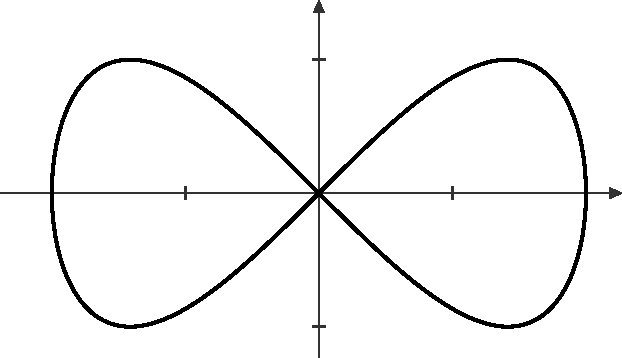
\includegraphics[width=0.7\textwidth]{figures/lemniscate.pdf}
            \caption{``$\infty$''或双纽线}
        \end{figure}
        显然$r_*$总是非零的, 所以$r$是一个浸入.
        并且我们也能发现$r$是一个单射.
        然而$r$不是一个嵌入: 作为$\mathbb{R}$的开子集, $(-\pi,\pi)$不是一个紧集, 但它在$r$下的像在$\mathbb{R}^2$的子空间拓扑下是一个紧集, 所以$r$不是一个同胚.
        有时候这个曲线也被称为\textit{双纽线}.
    \end{enumerate}
\end{eg}

按照我们之前的想法, 子流形是大流形的一个子集, 而且自己也是一个流形.
不过我们要求这个子集是要在大流形的拓扑下成为流形, 不然会出现双纽线那样自交等各种情况.
所以我们利用嵌入给出子流形的定义:
\begin{defn}
    设微分流形$M,N$满足$M\subset N$, 如果包含映射$\iota:M\to N$是一个嵌入, 那么就称$M$为$N$的\textbf{子流形}.
    $M$在$N$中的\textbf{余维度}定义为$\codim{M}=\dim{N}-\dim{M}$.
\end{defn}

对曲线曲面论而言, 最重要的是欧氏空间子流形, 尤其是\textit{曲线}与\textit{超曲面}.
我们引用~\parencite[8.7节定义1]{Zorich_MathAnal}~中引入$k$-维曲面所用的定义.
\begin{thm}
    设$S\subset\mathbb{R}^n$, 赋予了$\mathbb{R}^n$的子空间拓扑.
    如果对每一点$x_0\in S$都存在$\mathbb{R}^n$的一个邻域$U(x_0)$以及一个微分同胚$\varphi:U(x_0)\to I^n$将这个邻域映为$\mathbb{R}^n$中的$n$-维单位立方体$I^n=\{t\in\mathbb{R}^n||t^i|<1,i=1,\cdots,n\}$,
    并且满足集合$S\cap U(x_0)$的像是$\mathbb{R}^n$中由关系$t^{k+1}=\cdots=t^n=0$定义的$k$-维平面在$I^n$中的部分,
    那么$S$是$\mathbb{R}^n$的一个$k$-维子流形.
\end{thm}
\begin{proof}
    这基本上是把流形的定义说了一遍.
    由于$S$是$\mathbb{R}^n$的子空间, 所以自动是第二可数的Haussdorff空间.
    由子空间拓扑可知$S\cap U(x_0)$是$x_0$在$S$中的一个邻域, 按照假设它同胚于
    \[I^n\cap\mathbb{R}^k\times\{0\}=\{t\in\mathbb{R}^n||t^i|<1,i=1,\cdots,k,t^{k+1}=\cdots=t^n=0\}\]
    而这个集合又同胚于$\mathbb{R}^k$中的标准单位立方体$I^k$, 从而$x_0$的邻域同胚于$\mathbb{R}^k$中的开集.
    因此$S$是一个$k$维拓扑流形.
    而又由于假设, 所有同胚都是微分同胚, 所以转移函数都是光滑的.
    因此$S$有微分结构, 是一个微分流形.
    由于$S$的拓扑即为$\mathbb{R}^n$的子空间拓扑, 所以$S$是$\mathbb{R}^n$的子流形.
\end{proof}

\begin{defn}
    欧氏空间中的\textbf{曲线}指的是维度为$1$的子流形.
    欧氏空间中的\textbf{超曲面}指的是余维度为$1$的子流形, 特别地, $3$维欧氏空间中的超曲面会被直接称为\textbf{曲面}.
\end{defn}

实践中我们更多处理的是例~\ref{submanifold_eg} (2) 中的参数化曲面片.
对一般的浸入来说, 我们没有办法说明它是不是嵌入, 从而也不能说明曲面片是不是流形.
但是以下的定理可以保证在局部上每个浸入都是嵌入, 从而每一个曲面片在局部都是一个$2$维子流形, 或者说曲面.
\begin{thm}
    设$M,N$是微分流形, $f:M\to N$是光滑映射.
    那么$f$是一个浸入当且仅当$M$中的每一个点都有一个邻域$U$使得$f|U:U\to N$是一个嵌入.
\end{thm}
\begin{proof}
    \parencite[定理4.25]{Lee_IntroSmMani}.
\end{proof}

\section{向量场}
向量场是我们研究流形的主要工具之一, 本节我们讨论一些简单的有关向量场的性质.

\subsection*{向量场与微分映射}
\begin{defn}
    设$X:M\to TM$是一个光滑映射, 如果有$\pi\circ X=1_M$成立, 其中$1_M$是$M$到自身的恒等映射, 那么称$X$是$M$上的一个\textbf{向量场}.
\end{defn}
\begin{rem}
    我们讲一下这个定义是怎么回事.
    向量场实际上是希望在流形每一点的切空间处光滑地指派一个向量.
    为了描述光滑, 我们会直接定义一个光滑的映射$X:M\to TM$, 同时为了让点$p$处的向量$X_p$在$T_pM$中, 我们让$\pi\circ X=1_M$成立.
    如果套用传统的定义来说的话, 我们会取定一个坐标卡$(U,\varphi)$, 对任意一点$p\in U$, 我们指派一个切向量:
    \begin{equation}
        p\mapsto\left(p,\sum_{i}a^i\frac{\partial}{\partial x^i}\right)\label{vector field on coordinate}
    \end{equation}
    其中$a^i$是$M$上的函数.
    那么取$TM$的坐标卡$(U\times\mathbb{R}^n,\varphi\times\varphi_*)$可知
    \begin{align*}
        &(\varphi\times\varphi_*)\circ X\circ\varphi^{-1}:\mathbb{R}^n\to\mathbb{R}^n\times\mathbb{R}^n\\
        &u\mapsto\left(u,(a^1\circ\varphi^{-1})(u),\cdots,(a^n\circ\varphi^{-1})(u)\right)
    \end{align*}
    所以向量场$X$是光滑的当且仅当每个坐标分量函数是光滑的.
    同时, \eqref{vector field on coordinate}\\也给出了一个向量场在某组坐标卡下的具体表示.
\end{rem}
\begin{sym}
    我们用$\mathfrak{X}(M)$表示$M$上全体向量场的集合, 它是一个$\mathbb{R}$-向量空间.
    按照显然定义的运算, 它也是一个$C^\infty(M)$-模 (一种在环上的满足类似向量空间运算律的结构, 之后会在定义~\ref{def of left module}~正式遇到它).
\end{sym}
\begin{eg}
    对给定的坐标卡$(U,\varphi)$, $\dfrac{\partial}{\partial x^1},\dfrac{\partial}{\partial x^2},\cdots,\dfrac{\partial}{\partial x^n}$是$\mathfrak{X}(U)$中的$n$个向量场, 它们在每点$p$处的取值构成了$T_pU$的一组基.
    这样的一组向量场被称为一组\textbf{局部自然标架}.
    如果存在$\mathfrak{X}(M)$中的$n$个向量场满足它们在每点处的取值都构成切空间的一组基, 那么这组向量场称为$M$的一组\textbf{标架}, 同时我们称切丛$TM$是\textbf{平凡的}.
    容易注意到, 平凡的切丛$TM$总是同胚于$M\times\mathbb{R}^n$, 所以我们会将其称为是平凡的.
    这也再次说明了评注~\ref{local trivialization}~中将坐标卡称为局部平凡化的理由.
\end{eg}

向量场的一个特点是可以像微分一样作用在光滑函数上.
我们知道$p$点处的一个切向量$X_p$将一个光滑函数映成一个数, 那么一个向量场$X$在每一点都将一个光滑函数映成一个数,
因此我们有
\begin{prop}\label{vector field act}
    设$X\in\mathfrak{X}(M)$, 那么$X$诱导了$C^\infty(M)$到自身的一个映射.
    如果把$f$在映射下的像记作$Xf$, 那么这个映射定义为
    \[Xf(p)=X_p(f)\]
\end{prop}
\begin{proof}
    只需验证$Xf$是光滑的.
    而只需注意到在局部设$\displaystyle X=\sum_{i}a^i\dfrac{\partial}{\partial x^i}$, 那么有
    \[Xf=\sum_{i}a^i\frac{\partial f}{\partial x^i}\]
    从而由$a^i$的光滑性与光滑函数的线性性可知$Xf$是光滑的.
\end{proof}
反过来, 我们还有一个判别方法:
\begin{prop}
    如果$Y$是一个$C^\infty(M)$到自身的映射, 那么$Y$是$\mathfrak{X}(M)$中的向量场按命题~\ref{vector field act}~诱导出来的当且仅当它满足Leibniz法则, 即对任意$f,g\in C^\infty(M)$有$Y(fg)=fYg+gYf$.
\end{prop}
\begin{proof}
    如果$Y$是向量场诱导出来的, 那么它显然满足Leibniz法则.
    如果$Y$满足Leibniz法则, 考虑等式两侧在$p$点处的取值, 可知此时``$Y$作用+赋值$p$''相当于$T_pM$中的一个元素.
    收集所有的元素得到一个 (不一定连续的) 向量场$X$, $X$可以诱导出$Y$.
    我们还需要说明$X$是光滑的.
    设在局部有$\displaystyle X=\sum_{i}a^i\dfrac{\partial}{\partial x^i}$, 那么有
    \[Xx^i=a^i,\ i=1,2\cdots,n\]
    由假设, $X$将光滑函数映成光滑函数, 所以$a^i$都是光滑的, 从而$X$是光滑的.
\end{proof}

\subsection*{Lie括号}
对于两个向量场$X,Y$与光滑函数$f$, 我们知道$XYf=X(Yf)$仍然是一个光滑函数.
但$XY$的作用是向量场诱导出来的吗?
我们来验证$XY$是否满足Leibniz法则.
注意到
\begin{equation}
    \begin{aligned}
        XY(fg)&=X(fYg+gYf)\\
        &=fXYg+gXYf+XfYg+XgYf
    \end{aligned}\label{XY act}
\end{equation}
从而$XY$是不满足Leibniz法则的.
不过我们考虑反过来的$YX$:
\begin{equation}
    YX(fg)=fYXg+gYXf+XfYg+XgYf\label{YX act}
\end{equation}
那么只需要让~\eqref{XY act}~与~\eqref{YX act}~两式相减, 就可以发现$XY-YX$的作用满足Leibniz法则.
因此我们有
\begin{prop}
    对$X,Y\in\mathfrak{X}(M)$, $XY-YX$的作用可以由向量场诱导得到, 这个向量场记为$[X,Y]$, 称作$X,Y$的\textbf{Lie括号}.
\end{prop}
\begin{eg}
    \begin{enumerate}[(1)]
        \item 对局部的自然标架$\left\{\dfrac{\partial}{\partial x^1},\dfrac{\partial}{\partial x^2},\cdots,\dfrac{\partial}{\partial x^n}\right\}$, 总有
        \[\left[\frac{\partial}{\partial x^i},\frac{\partial}{\partial x^j}\right]=0\]
        这实际上是反映了求偏导可以交换顺序.
        \item 对于两个向量场$\displaystyle X=\sum_{i}a^i\dfrac{\partial}{\partial x^i},Y=\sum_{i}b^i\dfrac{\partial}{\partial x^i}$, 我们计算它们的Lie括号有
        \begin{align*}
            [X,Y]&=\sum_{i}\left(\sum_{j}a^j\frac{\partial}{\partial x^j}\right)b^i\frac{\partial}{\partial x^i}-\sum_{i}\left(\sum_{j}b^j\frac{\partial}{\partial x^j}\right)a^i\frac{\partial}{\partial x^i}\\
            &=\sum_{i,j}a^j\left(\frac{\partial b^i}{\partial x^j}\frac{\partial}{\partial x^i}+b^i\frac{\partial^2}{\partial x^i\partial x^j}\right)-\sum_{i,j}b^j\left(\frac{\partial a^i}{\partial x^j}\frac{\partial}{\partial x^i}+a^i\frac{\partial^2}{\partial x^i\partial x^j}\right)\\
            &=\sum_{i,j}\left(a^j\frac{\partial b^i}{\partial x^j}-b^j\frac{\partial a^i}{\partial x^j}\right)\frac{\partial}{\partial x^i}
        \end{align*}
        通过这个表达式也可以证明$[X,Y]$是一个向量场.
        实际操作中, 我们会更多用这个表达式来计算Lie括号.
    \end{enumerate}
\end{eg}

\begin{prop}[Lie括号的性质]\label{property of lie bracket}
    对任意$X,Y,Z\in\mathfrak{X}(M)$有
    \begin{enumerate}[{\upshape 1.}]
        \item \rmparen{双线性性} 对任意$a,b\in\mathbb{R}$有
        \begin{gather*}
            [aX+bY,Z]=a[X,Z]+b[Y,Z]\\
            [Z,aX+bY]=a[Z,X]+b[Z,Y]
        \end{gather*}
        \item \rmparen{反对称性} \[[X,Y]=-[Y,X]\]
        \item \rmparen{Jacobi恒等式} \[[X,[Y,Z]]+[Y,[Z,X]]+[Z,[X,Y]]=0\]
        \item 对$f,g\in C^\infty(M)$有
        \[[fX,gY]=fg[X,Y]+(fXg)Y-(gYf)X\]
    \end{enumerate}
\end{prop}
\begin{proof}
    这些都是直接的计算, 也可以参考~\parencite[命题8.28]{Lee_IntroSmMani}.
\end{proof}

命题~\ref{property of lie bracket}~的前3条性质可以用来公理化地定义\textit{Lie代数}, 向量场与Lie括号也是我们见到的第一个Lie代数.
我们在此就不展开了.

\subsection*{子流形与向量场}
除了流形自身上的向量场以外, 我们还要对子流形再定义一种向量场.
\begin{defn}
    设$M$是$\widetilde{M}$的子流形, $\widetilde{M}$中一个\textbf{沿$M$的向量场}为一个光滑映射$X:M\to T\widetilde{M}$, 满足$\pi\circ X=1_M$.
    $\widetilde{M}$中所有沿$M$的向量场的集合记为$\Gamma(T\widetilde{M}|_M)$\footnote{这个记号来自于向量丛的截面.}.
\end{defn}
\begin{rem}
    ``沿$M$的向量场''和``$M$上的向量场''是有区别的.
    对前者而言, 每点$p$处的切向量可以在$T_p\widetilde{M}$中取值, 而后者的切向量只能在$T_pM$中取值.
    例如对$\mathbb{R}^n$的子流形$S$而言, $\Gamma(T\mathbb{R}^n|S)$中的元素可以在$\mathbb{R}^n$中取值,
    而$\mathfrak{X}(S)$中的元素 (局部上) 只能在$\mathbb{R}^n$的某个子空间里取值.
\end{rem}
我们考虑一下$\mathbb{R}^n$中的超曲面$S$.
由于$\codim{S}=1,T_pS\oplus T_pS^\perp=\mathbb{R}^n$, 可知$\dim{T_pS^\perp}=1$.
从而每一点处存在两个单位法向量, 适当地选取其中一个, 我们希望可以得到$S$的\textbf{单位法向量场}.
但这并不总是能够做到的, 事实上, 这与我们之前提到的流形的定向有关.
\begin{thm}\label{orientable iff normal field}
    $\mathbb{R}^n$中的超曲面$S$上存在单位法向量场的充分必要条件是$S$可定向.
\end{thm}
\begin{proof}
    对$\mathbb{R}^n$中的两组基, 如果它们的过渡矩阵行列式为正, 那么称它们定向相同.
    否则称为定向相反.
    固定$\mathbb{R}^n$的一组规范正交基$\mathcal{O}$.\\
    \textit{必要性}.
    假设$N$是单位法向量场.
    考虑一组覆盖了$S$的图册$\{U_\alpha,\varphi_\alpha\}$, 并考察$U$中标架场$\left\{\dfrac{\partial}{\partial x^1},\cdots,\dfrac{\partial}{\partial x^{n-1}},N\right\}$的定向.
    由于每一点处的标架到$\mathcal{O}$的过渡矩阵行列式是连续的, 所以$U$中标架场的过渡矩阵行列式总是恒正或恒负, 从而局部标架场的定向是良定义的.
    此时如果$\left\{\dfrac{\partial}{\partial x^1},\cdots,\dfrac{\partial}{\partial x^{n-1}},N\right\}$与$\mathcal{O}$定向不同, 那么将$\varphi_\alpha$复合一个对称变换$(u^1,u^2,\cdots,u^n)\mapsto(-u^1,u^2,\cdots,u^n)$, 得到的新坐标卡下的标架场$\left\{-\dfrac{\partial}{\partial x^1},\cdots,\dfrac{\partial}{\partial x^{n-1}},N\right\}$便与$\mathcal{O}$定向相同.
    因此, 存在一组图册使得每个坐标卡的局部标架场定向都与$\mathcal{O}$相同.
    对坐标卡$(U_\alpha,\varphi_\alpha),(U_\beta,\varphi_\beta)$, 设它们的标架场到$\mathcal{O}$的过渡矩阵分别为$A,B$, 考虑这两个标架场之间的过渡矩阵, 注意到$N$是共同的一个向量, 有
    \begin{align*}
        0&<\det{A}\det{B^{-1}}\\
        &=\det\begin{bmatrix}
            (\varphi_\alpha)_*\circ(\varphi_\beta^{-1})_* & \\
             & 1
        \end{bmatrix}\\
        &=\det(\varphi_\alpha\circ\varphi_\beta^{-1})_*
    \end{align*}
    所以$S$可定向.\\
    \textit{充分性}.
    取定$S$的一个定向与决定这个定向的图册.
    对$p\in S$, 我们选取一个包含$p$的坐标卡$(U,\varphi)$, 并在$T_pS^\perp$中选择一个单位向量$N_p$使得标架$\left\{\left.\dfrac{\partial}{\partial x^1}\right|_p,\cdots,\left.\dfrac{\partial}{\partial x^{n-1}}\right|_p,N_p\right\}$与$\mathcal{O}$定向相同.
    我们证明$N_p$是良定义的.
    如果$(V,\psi)$是另一个坐标卡, 设$\left\{\left.\dfrac{\partial}{\partial x^1}\right|_p,\cdots,\left.\dfrac{\partial}{\partial x^{n-1}}\right|_p,N|_p\right\}$到$\mathcal{O}$的过渡矩阵为$A$, $\left\{\left.\dfrac{\partial}{\partial y^1}\right|_p,\cdots,\left.\dfrac{\partial}{\partial y^{n-1}}\right|_p,N|_p\right\}$到$\mathcal{O}$的过渡矩阵为$B$.
    那么有
    \begin{align*}
        \det{B}&=\det{
            \begin{bmatrix}
                (\psi\circ\varphi^{-1})_* & \\
                & 1
            \end{bmatrix}
        }\det{A}\\
        &>0
    \end{align*}
    因此是同向的, 从而$N_p$有良定义.
    我们最后需要说明$N$是光滑的.
    设局部标架场$\left\{\dfrac{\partial}{\partial x^1},\dfrac{\partial}{\partial x^2},\cdots,\dfrac{\partial}{\partial x^{n-1}}\right\}$在$\mathcal{O}:=\{e_1,\cdots,e_n\}$下的坐标为
    \[\frac{\partial}{\partial x^i}=\sum_{j}a^j_ie_j,\quad i=1,2,\cdots,n-1\]
    又设$\displaystyle N=\sum_{i}N^ie_i$, 那么由垂直关系知$(N^1,N^2,\cdots,N^n)$是线性方程组
    \begin{align*}
        \left\{\begin{array}{ccc}
            a^1_1x_1+a^2_1x_2+\cdots+a^n_1x_n & = & 0\\
            a^1_2x_1+a^2_2x_2+\cdots+a^n_2x_n & = & 0\\
            \cdots\cdots & & \\
            a^1_{n-1}x_1+a^2_{n-1}x_2+\cdots+a^n_{n-1}x_n & = & 0\\
        \end{array}\right.
    \end{align*}
    的解, 可以被代数函数表示, 所以一定是光滑的.
\end{proof} % 要是我来评论这一段, 我会说这人线性代数没学好

这是我们翻来覆去嚼了很多定义之后遇到的第一个真正的``定理''.

此外, 如果我们发散一下定理~\ref{orientable iff normal field}~的证明思路, 可以直觉出来一个结论:
可定向流形上面一定存在标架场, 从而切丛是平凡的.
但是目前我们还证明不了这件事情, 我们还需要等待单位分解定理的出场.

作为本章的结束, 我们来讨论在第~\ref{sect_of_mani}~节结尾处留下的问题, 即证明M\"{o}bius带是不可定向的.
\begin{eg}
    M\"{o}bius带是把一个纸条扭转一次, 然后粘合两端得到的.
    比较自然的方法是使用商拓扑 (也叫``手术''), 但我们在这里直接一些, 把M\"{o}bius带看成直纹面写参数方程.
    我们有
    \[r(u,v)=a(u)+vl(u)\]
    其中
    \begin{gather*}
        a(u)=a(\cos{2u},\sin{2u},0)\\
        l(u)=a(u)\cos{u}+(0,0,a\sin{u})\\
        u\in[0,\pi),v\in\left(-\frac{1}{2},\frac{1}{2}\right)
    \end{gather*}
    假如M\"{o}bius带可定向, 那么它有单位法向量场$N$, 不妨设$(a,0,0)$处取值为
    \begin{align*}
        \frac{r_u(0,0)\times r_v(0,0)}{|r_u(0,0)\times r_v(0,0)|}&=\frac{(0,2a,0)\times(a,0,0)}{2a^2}\\
        &=(0,0,-1)
    \end{align*}
    (回忆例~\ref{submanifold_eg}~(2) 中表示偏导数的记号)
    考虑$N$在准线$a(u)$上的限制, 按照连续性, 对任意$0\leq t<\pi$都有
    \begin{align*}
        N_{a(t)}&=\frac{r_u(t)\times r_v(t)}{|r_u(t)\times r_v(t)|}\\
        &=(r_u(t)\times r_v(t))^0
    \end{align*}
    但
    \begin{align*}
        \lim_{t\to\pi}N_{a(t)}&=\left(\lim_{t\to\pi}r_u(t)\times\lim_{t\to\pi}r_v(t)\right)^0\\
        &=((0,2a,0)\times(0,-a,0))^0\\
        &=(0,0,1)\\
        &\neq N_{a(0)}
    \end{align*}
    与连续性矛盾.
    所以M\"{o}bius带不可定向.
\end{eg}
\blank